% Options for packages loaded elsewhere
\PassOptionsToPackage{unicode}{hyperref}
\PassOptionsToPackage{hyphens}{url}
%
\documentclass[
]{article}
\usepackage{amsmath,amssymb}
\usepackage{iftex}
\ifPDFTeX
  \usepackage[T1]{fontenc}
  \usepackage[utf8]{inputenc}
  \usepackage{textcomp} % provide euro and other symbols
\else % if luatex or xetex
  \usepackage{unicode-math} % this also loads fontspec
  \defaultfontfeatures{Scale=MatchLowercase}
  \defaultfontfeatures[\rmfamily]{Ligatures=TeX,Scale=1}
\fi
\usepackage{lmodern}
\ifPDFTeX\else
  % xetex/luatex font selection
\fi
% Use upquote if available, for straight quotes in verbatim environments
\IfFileExists{upquote.sty}{\usepackage{upquote}}{}
\IfFileExists{microtype.sty}{% use microtype if available
  \usepackage[]{microtype}
  \UseMicrotypeSet[protrusion]{basicmath} % disable protrusion for tt fonts
}{}
\makeatletter
\@ifundefined{KOMAClassName}{% if non-KOMA class
  \IfFileExists{parskip.sty}{%
    \usepackage{parskip}
  }{% else
    \setlength{\parindent}{0pt}
    \setlength{\parskip}{6pt plus 2pt minus 1pt}}
}{% if KOMA class
  \KOMAoptions{parskip=half}}
\makeatother
\usepackage{xcolor}
\usepackage[margin=1in]{geometry}
\usepackage{color}
\usepackage{fancyvrb}
\newcommand{\VerbBar}{|}
\newcommand{\VERB}{\Verb[commandchars=\\\{\}]}
\DefineVerbatimEnvironment{Highlighting}{Verbatim}{commandchars=\\\{\}}
% Add ',fontsize=\small' for more characters per line
\usepackage{framed}
\definecolor{shadecolor}{RGB}{248,248,248}
\newenvironment{Shaded}{\begin{snugshade}}{\end{snugshade}}
\newcommand{\AlertTok}[1]{\textcolor[rgb]{0.94,0.16,0.16}{#1}}
\newcommand{\AnnotationTok}[1]{\textcolor[rgb]{0.56,0.35,0.01}{\textbf{\textit{#1}}}}
\newcommand{\AttributeTok}[1]{\textcolor[rgb]{0.13,0.29,0.53}{#1}}
\newcommand{\BaseNTok}[1]{\textcolor[rgb]{0.00,0.00,0.81}{#1}}
\newcommand{\BuiltInTok}[1]{#1}
\newcommand{\CharTok}[1]{\textcolor[rgb]{0.31,0.60,0.02}{#1}}
\newcommand{\CommentTok}[1]{\textcolor[rgb]{0.56,0.35,0.01}{\textit{#1}}}
\newcommand{\CommentVarTok}[1]{\textcolor[rgb]{0.56,0.35,0.01}{\textbf{\textit{#1}}}}
\newcommand{\ConstantTok}[1]{\textcolor[rgb]{0.56,0.35,0.01}{#1}}
\newcommand{\ControlFlowTok}[1]{\textcolor[rgb]{0.13,0.29,0.53}{\textbf{#1}}}
\newcommand{\DataTypeTok}[1]{\textcolor[rgb]{0.13,0.29,0.53}{#1}}
\newcommand{\DecValTok}[1]{\textcolor[rgb]{0.00,0.00,0.81}{#1}}
\newcommand{\DocumentationTok}[1]{\textcolor[rgb]{0.56,0.35,0.01}{\textbf{\textit{#1}}}}
\newcommand{\ErrorTok}[1]{\textcolor[rgb]{0.64,0.00,0.00}{\textbf{#1}}}
\newcommand{\ExtensionTok}[1]{#1}
\newcommand{\FloatTok}[1]{\textcolor[rgb]{0.00,0.00,0.81}{#1}}
\newcommand{\FunctionTok}[1]{\textcolor[rgb]{0.13,0.29,0.53}{\textbf{#1}}}
\newcommand{\ImportTok}[1]{#1}
\newcommand{\InformationTok}[1]{\textcolor[rgb]{0.56,0.35,0.01}{\textbf{\textit{#1}}}}
\newcommand{\KeywordTok}[1]{\textcolor[rgb]{0.13,0.29,0.53}{\textbf{#1}}}
\newcommand{\NormalTok}[1]{#1}
\newcommand{\OperatorTok}[1]{\textcolor[rgb]{0.81,0.36,0.00}{\textbf{#1}}}
\newcommand{\OtherTok}[1]{\textcolor[rgb]{0.56,0.35,0.01}{#1}}
\newcommand{\PreprocessorTok}[1]{\textcolor[rgb]{0.56,0.35,0.01}{\textit{#1}}}
\newcommand{\RegionMarkerTok}[1]{#1}
\newcommand{\SpecialCharTok}[1]{\textcolor[rgb]{0.81,0.36,0.00}{\textbf{#1}}}
\newcommand{\SpecialStringTok}[1]{\textcolor[rgb]{0.31,0.60,0.02}{#1}}
\newcommand{\StringTok}[1]{\textcolor[rgb]{0.31,0.60,0.02}{#1}}
\newcommand{\VariableTok}[1]{\textcolor[rgb]{0.00,0.00,0.00}{#1}}
\newcommand{\VerbatimStringTok}[1]{\textcolor[rgb]{0.31,0.60,0.02}{#1}}
\newcommand{\WarningTok}[1]{\textcolor[rgb]{0.56,0.35,0.01}{\textbf{\textit{#1}}}}
\usepackage{graphicx}
\makeatletter
\def\maxwidth{\ifdim\Gin@nat@width>\linewidth\linewidth\else\Gin@nat@width\fi}
\def\maxheight{\ifdim\Gin@nat@height>\textheight\textheight\else\Gin@nat@height\fi}
\makeatother
% Scale images if necessary, so that they will not overflow the page
% margins by default, and it is still possible to overwrite the defaults
% using explicit options in \includegraphics[width, height, ...]{}
\setkeys{Gin}{width=\maxwidth,height=\maxheight,keepaspectratio}
% Set default figure placement to htbp
\makeatletter
\def\fps@figure{htbp}
\makeatother
\setlength{\emergencystretch}{3em} % prevent overfull lines
\providecommand{\tightlist}{%
  \setlength{\itemsep}{0pt}\setlength{\parskip}{0pt}}
\setcounter{secnumdepth}{5}
\ifLuaTeX
  \usepackage{selnolig}  % disable illegal ligatures
\fi
\usepackage{bookmark}
\IfFileExists{xurl.sty}{\usepackage{xurl}}{} % add URL line breaks if available
\urlstyle{same}
\hypersetup{
  pdftitle={Survey Analysis: Math 3210 Project 1},
  pdfauthor={Noah G. Gallego},
  hidelinks,
  pdfcreator={LaTeX via pandoc}}

\title{Survey Analysis: Math 3210 Project 1}
\author{Noah G. Gallego}
\date{2024-11-11}

\begin{document}
\maketitle

{
\setcounter{tocdepth}{2}
\tableofcontents
}
\section{Introduction}\label{introduction}

In this project, we will analyze survey data collected from classmates
to gain insights into their financial habits and situations, including
budgeting methods, spending patterns, saving behaviors, and concerns
about debt. We'll conduct data cleaning and exploratory data analysis
(EDA) to identify trends and patterns within financial practices. Using
descriptive statistics, visualizations, and inferential analysis, we aim
to highlight relationships between financial behaviors and various
factors that may influence financial decision-making. This analysis will
provide a deeper understanding of the financial habits and challenges
among our peers.

\subsection{Load Libraries:}\label{load-libraries}

\begin{Shaded}
\begin{Highlighting}[]
\FunctionTok{library}\NormalTok{(dplyr)}
\FunctionTok{library}\NormalTok{(ggplot2)}
\FunctionTok{library}\NormalTok{(tm)}
\end{Highlighting}
\end{Shaded}

\begin{verbatim}
## Loading required package: NLP
\end{verbatim}

\begin{verbatim}
## 
## Attaching package: 'NLP'
\end{verbatim}

\begin{verbatim}
## The following object is masked from 'package:ggplot2':
## 
##     annotate
\end{verbatim}

\begin{verbatim}
## 
## Attaching package: 'tm'
\end{verbatim}

\begin{verbatim}
## The following object is masked from 'package:mosaic':
## 
##     inspect
\end{verbatim}

\begin{Shaded}
\begin{Highlighting}[]
\FunctionTok{library}\NormalTok{(wordcloud)}
\end{Highlighting}
\end{Shaded}

\begin{verbatim}
## Loading required package: RColorBrewer
\end{verbatim}

\begin{Shaded}
\begin{Highlighting}[]
\FunctionTok{library}\NormalTok{(RColorBrewer)}
\FunctionTok{library}\NormalTok{(reshape2)}
\end{Highlighting}
\end{Shaded}

\begin{verbatim}
## 
## Attaching package: 'reshape2'
\end{verbatim}

\begin{verbatim}
## The following object is masked from 'package:tidyr':
## 
##     smiths
\end{verbatim}

\begin{Shaded}
\begin{Highlighting}[]
\FunctionTok{library}\NormalTok{(cluster)}
\FunctionTok{library}\NormalTok{(ggcorrplot)}
\FunctionTok{library}\NormalTok{(tidyr)}
\FunctionTok{library}\NormalTok{(tidyverse)}
\FunctionTok{library}\NormalTok{(stats)}
\FunctionTok{library}\NormalTok{(caret)}
\end{Highlighting}
\end{Shaded}

\begin{verbatim}
## 
## Attaching package: 'caret'
\end{verbatim}

\begin{verbatim}
## The following object is masked from 'package:mosaic':
## 
##     dotPlot
\end{verbatim}

\begin{verbatim}
## The following object is masked from 'package:purrr':
## 
##     lift
\end{verbatim}

\subsection{Load Data \& Basic Cleaning}\label{load-data-basic-cleaning}

\begin{Shaded}
\begin{Highlighting}[]
\CommentTok{\# Load the DataFrame}
\NormalTok{df }\OtherTok{=} \FunctionTok{read.csv}\NormalTok{(}\StringTok{"ProData.csv"}\NormalTok{, }\AttributeTok{header =} \ConstantTok{TRUE}\NormalTok{)}

\CommentTok{\# Remove Unnecessary Rows}
\NormalTok{df }\OtherTok{=}\NormalTok{ df[}\SpecialCharTok{{-}}\FunctionTok{c}\NormalTok{(}\DecValTok{1}\NormalTok{, }\DecValTok{2}\NormalTok{), ]}

\CommentTok{\# Select Needed Cols}
\NormalTok{cols }\OtherTok{=} \FunctionTok{c}\NormalTok{(}\StringTok{"RecordedDate"}\NormalTok{, }\StringTok{"LocationLatitude"}\NormalTok{, }\StringTok{"LocationLongitude"}\NormalTok{, }\StringTok{"Question.One."}\NormalTok{, }\StringTok{"Question.Two.\_1"}\NormalTok{, }\StringTok{"Question.3."}\NormalTok{, }\StringTok{"Question.4\_1"}\NormalTok{, }\StringTok{"Question.5"}\NormalTok{, }\StringTok{"Question.6"}\NormalTok{, }\StringTok{"Question.7"}\NormalTok{, }\StringTok{"Question.8"}\NormalTok{, }\StringTok{"Question.9"}\NormalTok{, }\StringTok{"Question.10"}\NormalTok{, }\StringTok{"Question.11"}\NormalTok{)}
\NormalTok{df }\OtherTok{=}\NormalTok{ df[, cols]}
\NormalTok{df }\OtherTok{=}\NormalTok{ df }\SpecialCharTok{\%\textgreater{}\%}
  \FunctionTok{rename}\NormalTok{(}
    \AttributeTok{Date\_Recorded =}\NormalTok{ RecordedDate,}
    \AttributeTok{Latitude =}\NormalTok{ LocationLatitude,}
    \AttributeTok{Longitude =}\NormalTok{ LocationLongitude,}
    \AttributeTok{Budget\_Management\_Method =}\NormalTok{ Question.One.,}
    \AttributeTok{Financial\_Confidence =}\NormalTok{ Question.Two.\_1,}
    \AttributeTok{Student\_Loans =}\NormalTok{ Question.}\FloatTok{3.}\NormalTok{,}
    \AttributeTok{Student\_Debt\_Concern =}\NormalTok{ Question}\FloatTok{.4}\NormalTok{\_1,}
    \AttributeTok{Future\_Financial\_Decision\_Impact =}\NormalTok{ Question}\FloatTok{.5}\NormalTok{,}
    \AttributeTok{Biggest\_Expense =}\NormalTok{ Question}\FloatTok{.6}\NormalTok{,}
    \AttributeTok{Employment\_Status =}\NormalTok{ Question}\FloatTok{.7}\NormalTok{,}
    \AttributeTok{Saving\_For\_Future\_Expenses =}\NormalTok{ Question}\FloatTok{.8}\NormalTok{,}
    \AttributeTok{Saving\_For\_Retirement =}\NormalTok{ Question}\FloatTok{.9}\NormalTok{,}
    \AttributeTok{Financial\_Independence\_Confidence =}\NormalTok{ Question}\FloatTok{.10}\NormalTok{,}
    \AttributeTok{Job\_Confidence\_Post\_Graduation =}\NormalTok{ Question}\FloatTok{.11}
\NormalTok{  )}

\CommentTok{\# Display First Few Rows}
\NormalTok{df}
\end{Highlighting}
\end{Shaded}

\begin{verbatim}
##          Date_Recorded Latitude Longitude     Budget_Management_Method
## 3  2024-10-03 00:31:22  35.3965 -119.1268        Using a budgeting app
## 4  2024-10-03 00:39:15  35.3407 -119.0596        Using a budgeting app
## 5  2024-10-18 23:03:12  33.7046 -117.8739      I don't manage a budget
## 6  2024-10-19 21:23:19  35.7768 -119.2414 Manually (notebook or Excel)
## 7  2024-10-19 21:32:32  35.3044 -119.1031          No budgeting at all
## 8  2024-10-20 20:39:40  35.3878  -118.936      I don't manage a budget
## 9  2024-10-20 22:28:16  35.3044 -119.1031      I don't manage a budget
## 10 2024-10-20 23:29:36  45.8491 -119.7143          No budgeting at all
## 11 2024-10-21 00:06:31  35.3879 -118.9861          No budgeting at all
## 12 2024-10-21 13:16:43  35.4145 -119.0403 Manually (notebook or Excel)
## 13 2024-10-22 23:02:49  35.3044 -119.1031 Manually (notebook or Excel)
##    Financial_Confidence Student_Loans Student_Debt_Concern
## 3                     5            No                    5
## 4                     3            No                    4
## 5                     4            No                    3
## 6                                  No                    1
## 7                     2            No                    0
## 8                     4            No                     
## 9                     4            No                    0
## 10                    4            No                    4
## 11                    3            No                     
## 12                    5           Yes                    5
## 13                    3           Yes                    4
##                                                                                                                                              Future_Financial_Decision_Impact
## 3                          I think that student debt heavily impacts future financial decisions. Loans affect credit for good or bad depending on if you pay your loans off. 
## 4                                                                                                       Student debt will have a big impact on my financial future decisions.
## 5                                                                                                                                                              BuYiNg A hoMe 
## 6                               Too in my own head. conscious of my spending habits. inclined to save and pay off debt which i may have to sacrifice days of food and luxury.
## 7  I think student debt will have me try to save more money and buy only what I need. This means being more careful with spending on things I want rather than things I need.
## 8                                                                                                                          If I had student debt, I believe it would affect. 
## 9                                                                     I'm not taking on any debt which will be helpful in the future as it's one less expense to worry about.
## 10                                                                                                                                                                        Nah
## 11                                                                                                                                                          I don’t have any 
## 12                                                                       They can be paid off immediately after graduation so they will not affect future financial decisions
## 13                                                                                                          I plan to pay it off quickly after graduation, so not much I hope
##    Biggest_Expense Employment_Status Saving_For_Future_Expenses
## 3   Groceries/Food   Yes, part-time.                        Yes
## 4    Entertainment   Yes, part-time.                        Yes
## 5    Entertainment                No                         No
## 6   Groceries/Food   Yes, part-time.                         No
## 7            Other                No                         No
## 8    Rent/Mortgage   Yes, part-time.                        Yes
## 9   Transportation   Yes, part-time.                         No
## 10  Groceries/Food   Yes, full-time.                        Yes
## 11   Rent/Mortgage   Yes, part-time.                        Yes
## 12   Rent/Mortgage   Yes, part-time.                        Yes
## 13   Rent/Mortgage   Yes, part-time.                        Yes
##    Saving_For_Retirement Financial_Independence_Confidence
## 3                    Yes                         Confident
## 4                    Yes                         Confident
## 5                     No                     Not Confident
## 6                    Yes                         Confident
## 7                     No                         Confident
## 8                     No                         Confident
## 9                     No                         Confident
## 10                   Yes                         Confident
## 11                    No                     Not Confident
## 12                   Yes                     Not Confident
## 13                    No                         Confident
##    Job_Confidence_Post_Graduation
## 3                   Not Confident
## 4                   Not Confident
## 5                   Not Confident
## 6                   Not Confident
## 7                       Confident
## 8                       Confident
## 9                       Confident
## 10                      Confident
## 11                      Confident
## 12                      Confident
## 13                      Confident
\end{verbatim}

\subsection{Further Cleaning}\label{further-cleaning}

\begin{Shaded}
\begin{Highlighting}[]
\CommentTok{\# Convert Cols to Ints where Needed}
\NormalTok{df }\OtherTok{=}\NormalTok{ df }\SpecialCharTok{\%\textgreater{}\%}
  \FunctionTok{mutate}\NormalTok{(}\FunctionTok{across}\NormalTok{(}\FunctionTok{c}\NormalTok{(Latitude, Longitude, Financial\_Confidence, Student\_Debt\_Concern), as.numeric))}

\CommentTok{\# Convert Response to DT}
\NormalTok{df}\SpecialCharTok{$}\NormalTok{Date\_Recorded }\OtherTok{=} \FunctionTok{as.Date}\NormalTok{(df}\SpecialCharTok{$}\NormalTok{Date\_Recorded)}

\CommentTok{\# Convert Binary Responses to 1/0 For Analysis}
\NormalTok{df }\OtherTok{=}\NormalTok{ df }\SpecialCharTok{\%\textgreater{}\%}
  \FunctionTok{mutate}\NormalTok{(}
    \AttributeTok{Student\_Loans =} \FunctionTok{ifelse}\NormalTok{(}\FunctionTok{trimws}\NormalTok{(}\FunctionTok{tolower}\NormalTok{(Student\_Loans)) }\SpecialCharTok{==} \StringTok{"yes"}\NormalTok{, }\DecValTok{1}\NormalTok{, }\DecValTok{0}\NormalTok{),}
    \AttributeTok{Financial\_Independence\_Confidence =} \FunctionTok{ifelse}\NormalTok{(}\FunctionTok{trimws}\NormalTok{(}\FunctionTok{tolower}\NormalTok{(Financial\_Independence\_Confidence)) }\SpecialCharTok{==} \StringTok{"confident"}\NormalTok{, }\DecValTok{1}\NormalTok{, }\DecValTok{0}\NormalTok{),}
    \AttributeTok{Job\_Confidence\_Post\_Graduation =} \FunctionTok{ifelse}\NormalTok{(}\FunctionTok{trimws}\NormalTok{(}\FunctionTok{tolower}\NormalTok{(Job\_Confidence\_Post\_Graduation)) }\SpecialCharTok{==} \StringTok{"confident"}\NormalTok{, }\DecValTok{1}\NormalTok{, }\DecValTok{0}\NormalTok{),}
    \AttributeTok{Saving\_For\_Future\_Expenses =} \FunctionTok{ifelse}\NormalTok{(}\FunctionTok{trimws}\NormalTok{(}\FunctionTok{tolower}\NormalTok{(Saving\_For\_Future\_Expenses)) }\SpecialCharTok{==} \StringTok{"yes"}\NormalTok{, }\DecValTok{1}\NormalTok{, }\DecValTok{0}\NormalTok{),}
    \AttributeTok{Saving\_For\_Retirement =} \FunctionTok{ifelse}\NormalTok{(}\FunctionTok{trimws}\NormalTok{(}\FunctionTok{tolower}\NormalTok{(Saving\_For\_Retirement)) }\SpecialCharTok{==} \StringTok{"yes"}\NormalTok{, }\DecValTok{1}\NormalTok{, }\DecValTok{0}\NormalTok{),}
    \AttributeTok{Employment\_Status =} \FunctionTok{ifelse}\NormalTok{(}\FunctionTok{trimws}\NormalTok{(}\FunctionTok{tolower}\NormalTok{(Employment\_Status)) }\SpecialCharTok{==} \StringTok{"yes, part{-}time"} \SpecialCharTok{|} 
                               \FunctionTok{trimws}\NormalTok{(}\FunctionTok{tolower}\NormalTok{(Employment\_Status)) }\SpecialCharTok{==} \StringTok{"yes, full{-}time"}\NormalTok{, }\DecValTok{1}\NormalTok{, }\DecValTok{0}\NormalTok{)}
\NormalTok{  )}

\CommentTok{\# Function to calculate the mode}
\NormalTok{get\_mode }\OtherTok{=} \ControlFlowTok{function}\NormalTok{(x) \{}
\NormalTok{  unique\_x }\OtherTok{=} \FunctionTok{na.omit}\NormalTok{(x)  }\CommentTok{\# Remove NA values}
\NormalTok{  unique\_x[}\FunctionTok{which.max}\NormalTok{(}\FunctionTok{tabulate}\NormalTok{(}\FunctionTok{match}\NormalTok{(x, unique\_x)))]}
\NormalTok{\}}

\CommentTok{\# Replace NAs with mode for each column}
\NormalTok{df }\OtherTok{=}\NormalTok{ df }\SpecialCharTok{\%\textgreater{}\%}
  \FunctionTok{mutate}\NormalTok{(}\FunctionTok{across}\NormalTok{(}\FunctionTok{everything}\NormalTok{(), }\SpecialCharTok{\textasciitilde{}} \FunctionTok{ifelse}\NormalTok{(}\FunctionTok{is.na}\NormalTok{(.), }\FunctionTok{get\_mode}\NormalTok{(.), .)))}

\CommentTok{\# Re{-}Display Dataframe}
\FunctionTok{head}\NormalTok{(df)}
\end{Highlighting}
\end{Shaded}

\begin{verbatim}
##   Date_Recorded Latitude Longitude     Budget_Management_Method
## 3         19999  35.3965 -119.1268        Using a budgeting app
## 4         19999  35.3407 -119.0596        Using a budgeting app
## 5         20014  33.7046 -117.8739      I don't manage a budget
## 6         20015  35.7768 -119.2414 Manually (notebook or Excel)
## 7         20015  35.3044 -119.1031          No budgeting at all
## 8         20016  35.3878 -118.9360      I don't manage a budget
##   Financial_Confidence Student_Loans Student_Debt_Concern
## 3                    5             0                    5
## 4                    3             0                    4
## 5                    4             0                    3
## 6                    4             0                    1
## 7                    2             0                    0
## 8                    4             0                    4
##                                                                                                                                             Future_Financial_Decision_Impact
## 3                         I think that student debt heavily impacts future financial decisions. Loans affect credit for good or bad depending on if you pay your loans off. 
## 4                                                                                                      Student debt will have a big impact on my financial future decisions.
## 5                                                                                                                                                             BuYiNg A hoMe 
## 6                              Too in my own head. conscious of my spending habits. inclined to save and pay off debt which i may have to sacrifice days of food and luxury.
## 7 I think student debt will have me try to save more money and buy only what I need. This means being more careful with spending on things I want rather than things I need.
## 8                                                                                                                         If I had student debt, I believe it would affect. 
##   Biggest_Expense Employment_Status Saving_For_Future_Expenses
## 3  Groceries/Food                 0                          1
## 4   Entertainment                 0                          1
## 5   Entertainment                 0                          0
## 6  Groceries/Food                 0                          0
## 7           Other                 0                          0
## 8   Rent/Mortgage                 0                          1
##   Saving_For_Retirement Financial_Independence_Confidence
## 3                     1                                 1
## 4                     1                                 1
## 5                     0                                 0
## 6                     1                                 1
## 7                     0                                 1
## 8                     0                                 1
##   Job_Confidence_Post_Graduation
## 3                              0
## 4                              0
## 5                              0
## 6                              0
## 7                              1
## 8                              1
\end{verbatim}

\subsection{Exploratory Data Analysis
(EDA)}\label{exploratory-data-analysis-eda}

\subsubsection{Descriptive Statistics}\label{descriptive-statistics}

\begin{Shaded}
\begin{Highlighting}[]
\CommentTok{\# Summary Statistics}
\FunctionTok{summary}\NormalTok{(df)}
\end{Highlighting}
\end{Shaded}

\begin{verbatim}
##  Date_Recorded      Latitude       Longitude      Budget_Management_Method
##  Min.   :19999   Min.   :33.70   Min.   :-119.7   Length:11               
##  1st Qu.:20014   1st Qu.:35.30   1st Qu.:-119.1   Class :character        
##  Median :20016   Median :35.39   Median :-119.1   Mode  :character        
##  Mean   :20013   Mean   :36.20   Mean   :-119.0                           
##  3rd Qu.:20016   3rd Qu.:35.41   3rd Qu.:-119.0                           
##  Max.   :20018   Max.   :45.85   Max.   :-117.9                           
##  Financial_Confidence Student_Loans    Student_Debt_Concern
##  Min.   :2.000        Min.   :0.0000   Min.   :0.000       
##  1st Qu.:3.000        1st Qu.:0.0000   1st Qu.:2.000       
##  Median :4.000        Median :0.0000   Median :4.000       
##  Mean   :3.727        Mean   :0.1818   Mean   :3.091       
##  3rd Qu.:4.000        3rd Qu.:0.0000   3rd Qu.:4.000       
##  Max.   :5.000        Max.   :1.0000   Max.   :5.000       
##  Future_Financial_Decision_Impact Biggest_Expense    Employment_Status
##  Length:11                        Length:11          Min.   :0        
##  Class :character                 Class :character   1st Qu.:0        
##  Mode  :character                 Mode  :character   Median :0        
##                                                      Mean   :0        
##                                                      3rd Qu.:0        
##                                                      Max.   :0        
##  Saving_For_Future_Expenses Saving_For_Retirement
##  Min.   :0.0000             Min.   :0.0000       
##  1st Qu.:0.0000             1st Qu.:0.0000       
##  Median :1.0000             Median :0.0000       
##  Mean   :0.6364             Mean   :0.4545       
##  3rd Qu.:1.0000             3rd Qu.:1.0000       
##  Max.   :1.0000             Max.   :1.0000       
##  Financial_Independence_Confidence Job_Confidence_Post_Graduation
##  Min.   :0.0000                    Min.   :0.0000                
##  1st Qu.:0.5000                    1st Qu.:0.0000                
##  Median :1.0000                    Median :1.0000                
##  Mean   :0.7273                    Mean   :0.6364                
##  3rd Qu.:1.0000                    3rd Qu.:1.0000                
##  Max.   :1.0000                    Max.   :1.0000
\end{verbatim}

\begin{Shaded}
\begin{Highlighting}[]
\CommentTok{\# Mean, Median, Mode, Standard Deviation for Numerical Columns}
\NormalTok{mean\_values }\OtherTok{=} \FunctionTok{sapply}\NormalTok{(df }\SpecialCharTok{\%\textgreater{}\%} \FunctionTok{select\_if}\NormalTok{(is.numeric), mean, }\AttributeTok{na.rm =} \ConstantTok{TRUE}\NormalTok{)}
\NormalTok{median\_values }\OtherTok{=} \FunctionTok{sapply}\NormalTok{(df }\SpecialCharTok{\%\textgreater{}\%} \FunctionTok{select\_if}\NormalTok{(is.numeric), median, }\AttributeTok{na.rm =} \ConstantTok{TRUE}\NormalTok{)}
\NormalTok{mode\_values }\OtherTok{=} \FunctionTok{sapply}\NormalTok{(df }\SpecialCharTok{\%\textgreater{}\%} \FunctionTok{select\_if}\NormalTok{(is.numeric), get\_mode)}
\NormalTok{std\_dev\_values }\OtherTok{=} \FunctionTok{sapply}\NormalTok{(df }\SpecialCharTok{\%\textgreater{}\%} \FunctionTok{select\_if}\NormalTok{(is.numeric), sd, }\AttributeTok{na.rm =} \ConstantTok{TRUE}\NormalTok{)}

\FunctionTok{list}\NormalTok{(}\AttributeTok{mean =}\NormalTok{ mean\_values, }\AttributeTok{median =}\NormalTok{ median\_values, }\AttributeTok{mode =}\NormalTok{ mode\_values, }\AttributeTok{sd =}\NormalTok{ std\_dev\_values)}
\end{Highlighting}
\end{Shaded}

\begin{verbatim}
## $mean
##                     Date_Recorded                          Latitude 
##                     20012.9090909                        36.1973727 
##                         Longitude              Financial_Confidence 
##                      -119.0261545                         3.7272727 
##                     Student_Loans              Student_Debt_Concern 
##                         0.1818182                         3.0909091 
##                 Employment_Status        Saving_For_Future_Expenses 
##                         0.0000000                         0.6363636 
##             Saving_For_Retirement Financial_Independence_Confidence 
##                         0.4545455                         0.7272727 
##    Job_Confidence_Post_Graduation 
##                         0.6363636 
## 
## $median
##                     Date_Recorded                          Latitude 
##                        20016.0000                           35.3878 
##                         Longitude              Financial_Confidence 
##                         -119.1031                            4.0000 
##                     Student_Loans              Student_Debt_Concern 
##                            0.0000                            4.0000 
##                 Employment_Status        Saving_For_Future_Expenses 
##                            0.0000                            1.0000 
##             Saving_For_Retirement Financial_Independence_Confidence 
##                            0.0000                            1.0000 
##    Job_Confidence_Post_Graduation 
##                            1.0000 
## 
## $mode
##                     Date_Recorded                          Latitude 
##                        20016.0000                           35.3044 
##                         Longitude              Financial_Confidence 
##                         -119.1031                            4.0000 
##                     Student_Loans              Student_Debt_Concern 
##                            0.0000                            4.0000 
##                 Employment_Status        Saving_For_Future_Expenses 
##                            0.0000                            1.0000 
##             Saving_For_Retirement Financial_Independence_Confidence 
##                            0.0000                            1.0000 
##    Job_Confidence_Post_Graduation 
##                            1.0000 
## 
## $sd
##                     Date_Recorded                          Latitude 
##                         6.9635414                         3.2440356 
##                         Longitude              Financial_Confidence 
##                         0.4343394                         0.9045340 
##                     Student_Loans              Student_Debt_Concern 
##                         0.4045199                         1.8683975 
##                 Employment_Status        Saving_For_Future_Expenses 
##                         0.0000000                         0.5045250 
##             Saving_For_Retirement Financial_Independence_Confidence 
##                         0.5222330                         0.4670994 
##    Job_Confidence_Post_Graduation 
##                         0.5045250
\end{verbatim}

\subsubsection{Missing Values Analysis}\label{missing-values-analysis}

\begin{Shaded}
\begin{Highlighting}[]
\CommentTok{\# Check for Missing Values}
\NormalTok{missing\_values }\OtherTok{=} \FunctionTok{colSums}\NormalTok{(}\FunctionTok{is.na}\NormalTok{(df))}
\FunctionTok{print}\NormalTok{(missing\_values)}
\end{Highlighting}
\end{Shaded}

\begin{verbatim}
##                     Date_Recorded                          Latitude 
##                                 0                                 0 
##                         Longitude          Budget_Management_Method 
##                                 0                                 0 
##              Financial_Confidence                     Student_Loans 
##                                 0                                 0 
##              Student_Debt_Concern  Future_Financial_Decision_Impact 
##                                 0                                 0 
##                   Biggest_Expense                 Employment_Status 
##                                 0                                 0 
##        Saving_For_Future_Expenses             Saving_For_Retirement 
##                                 0                                 0 
## Financial_Independence_Confidence    Job_Confidence_Post_Graduation 
##                                 0                                 0
\end{verbatim}

\subsubsection{Visualizations}\label{visualizations}

\paragraph{Financial Confidence
Distribution}\label{financial-confidence-distribution}

\begin{Shaded}
\begin{Highlighting}[]
\FunctionTok{ggplot}\NormalTok{(df, }\FunctionTok{aes}\NormalTok{(}\AttributeTok{x =}\NormalTok{ Financial\_Confidence)) }\SpecialCharTok{+}
  \FunctionTok{geom\_histogram}\NormalTok{(}\AttributeTok{binwidth =} \DecValTok{1}\NormalTok{, }\AttributeTok{fill =} \StringTok{"blue"}\NormalTok{, }\AttributeTok{color =} \StringTok{"black"}\NormalTok{) }\SpecialCharTok{+}
  \FunctionTok{labs}\NormalTok{(}\AttributeTok{title =} \StringTok{"Financial Confidence Distribution (1 = Low, 5 = High)"}\NormalTok{, }\AttributeTok{x =} \StringTok{"Financial Confidence"}\NormalTok{, }\AttributeTok{y =} \StringTok{"Frequency"}\NormalTok{)}
\end{Highlighting}
\end{Shaded}

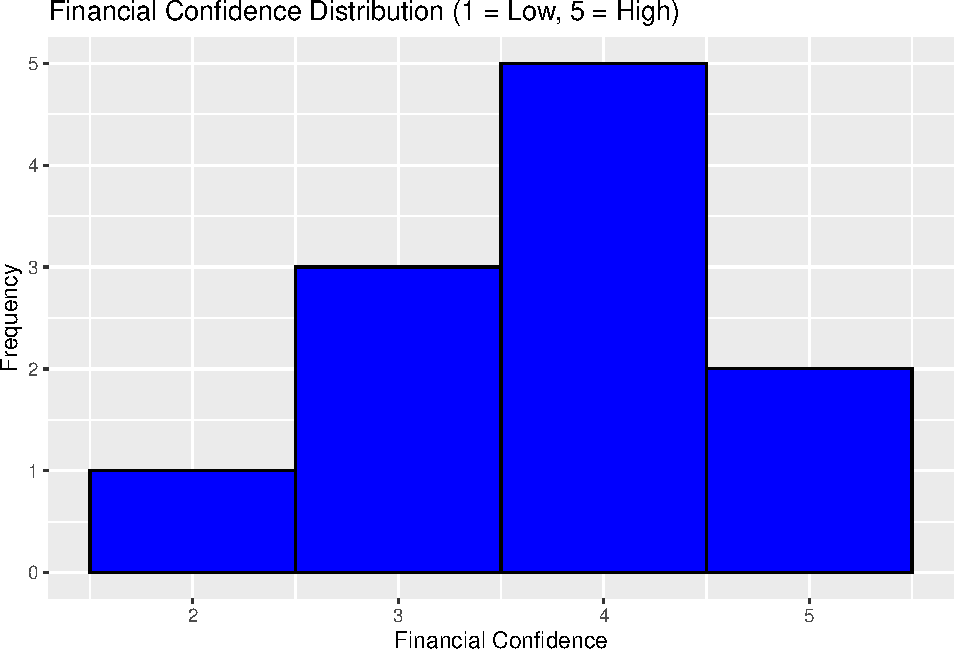
\includegraphics{Project1_files/figure-latex/unnamed-chunk-6-1.pdf}

\paragraph{Employment Status
Distribution}\label{employment-status-distribution}

\begin{Shaded}
\begin{Highlighting}[]
\CommentTok{\# Bar Plot for Employment Status}
\FunctionTok{ggplot}\NormalTok{(df, }\FunctionTok{aes}\NormalTok{(}\AttributeTok{x =} \FunctionTok{as.factor}\NormalTok{(Employment\_Status))) }\SpecialCharTok{+}
  \FunctionTok{geom\_bar}\NormalTok{(}\AttributeTok{fill =} \StringTok{"orange"}\NormalTok{, }\AttributeTok{color =} \StringTok{"black"}\NormalTok{) }\SpecialCharTok{+}
  \FunctionTok{labs}\NormalTok{(}\AttributeTok{title =} \StringTok{"Employment Status Distribution"}\NormalTok{, }\AttributeTok{x =} \StringTok{"Employment Status (0 = Unemployed, 1 = Employed)"}\NormalTok{, }\AttributeTok{y =} \StringTok{"Count"}\NormalTok{)}
\end{Highlighting}
\end{Shaded}

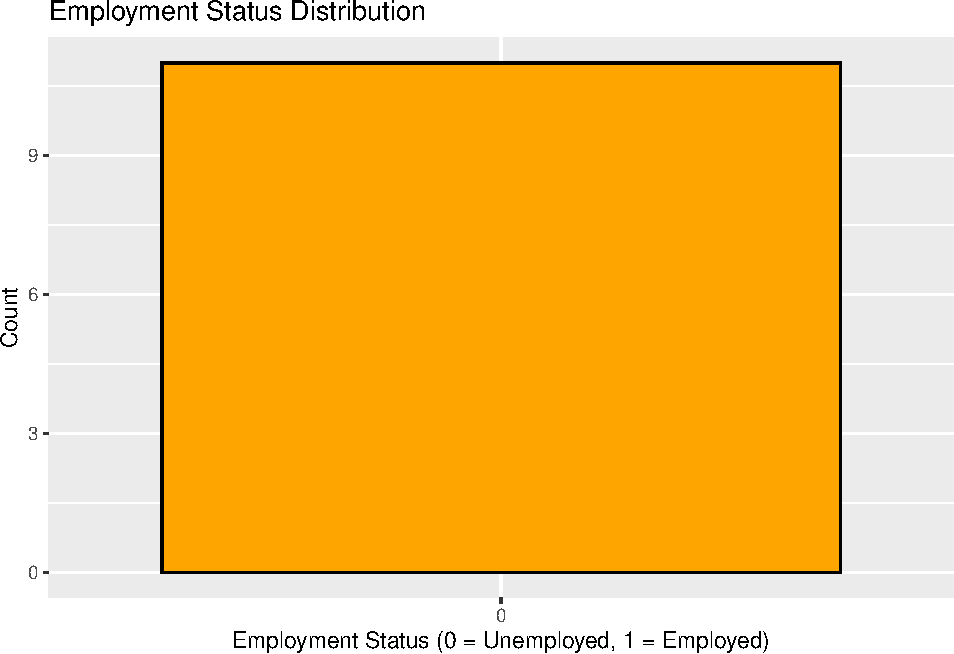
\includegraphics{Project1_files/figure-latex/unnamed-chunk-7-1.pdf}

\paragraph{Correlation Analysis}\label{correlation-analysis}

\begin{Shaded}
\begin{Highlighting}[]
\CommentTok{\# Correlation Plot (for numerical variables)}
\NormalTok{numeric\_cols }\OtherTok{=}\NormalTok{ df }\SpecialCharTok{\%\textgreater{}\%} \FunctionTok{select\_if}\NormalTok{(is.numeric)}
\NormalTok{correlation\_matrix }\OtherTok{=} \FunctionTok{cor}\NormalTok{(numeric\_cols, }\AttributeTok{use =} \StringTok{"complete.obs"}\NormalTok{)}
\end{Highlighting}
\end{Shaded}

\begin{verbatim}
## Warning in cor(numeric_cols, use = "complete.obs"): the standard deviation is
## zero
\end{verbatim}

\begin{Shaded}
\begin{Highlighting}[]
\FunctionTok{ggcorrplot}\NormalTok{(correlation\_matrix, }\AttributeTok{lab =} \ConstantTok{TRUE}\NormalTok{, }\AttributeTok{title =} \StringTok{"Correlation Heatmap"}\NormalTok{)}
\end{Highlighting}
\end{Shaded}

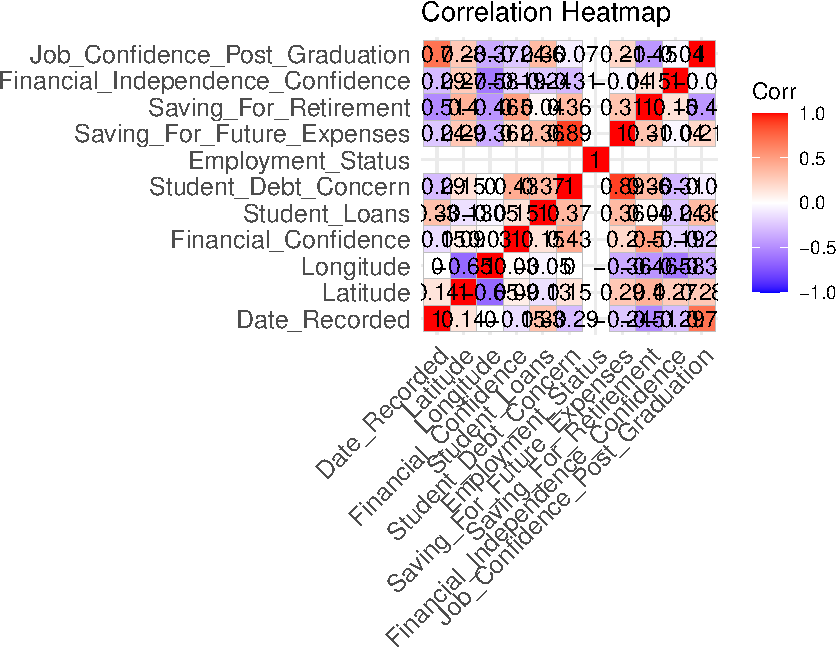
\includegraphics{Project1_files/figure-latex/unnamed-chunk-8-1.pdf}

\paragraph{Financial Confidence vs.~Student Debt
Concern}\label{financial-confidence-vs.-student-debt-concern}

\begin{Shaded}
\begin{Highlighting}[]
\CommentTok{\# Scatter Plot of Financial Confidence vs. Student Debt Concern}
\FunctionTok{ggplot}\NormalTok{(df, }\FunctionTok{aes}\NormalTok{(}\AttributeTok{x =}\NormalTok{ Financial\_Confidence, }\AttributeTok{y =}\NormalTok{ Student\_Debt\_Concern)) }\SpecialCharTok{+}
  \FunctionTok{geom\_point}\NormalTok{(}\AttributeTok{color =} \StringTok{"darkgreen"}\NormalTok{) }\SpecialCharTok{+}
  \FunctionTok{labs}\NormalTok{(}\AttributeTok{title =} \StringTok{"Scatter Plot of Financial Confidence vs Student Debt Concern"}\NormalTok{,}
       \AttributeTok{x =} \StringTok{"Financial Confidence"}\NormalTok{, }\AttributeTok{y =} \StringTok{"Student Debt Concern"}\NormalTok{)}
\end{Highlighting}
\end{Shaded}

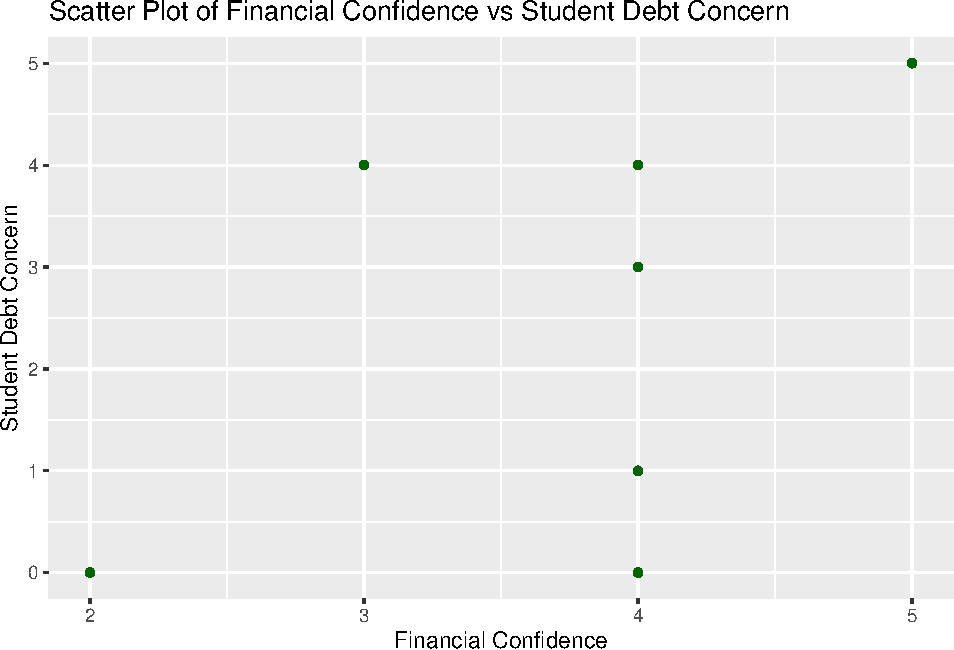
\includegraphics{Project1_files/figure-latex/unnamed-chunk-9-1.pdf}

\subsubsection{Additional
Visualizations}\label{additional-visualizations}

\paragraph{Budget Management Method
Distribution}\label{budget-management-method-distribution}

\begin{Shaded}
\begin{Highlighting}[]
\CommentTok{\# Bar Plot for Budget Management Methods}
\FunctionTok{ggplot}\NormalTok{(df, }\FunctionTok{aes}\NormalTok{(}\AttributeTok{x =}\NormalTok{ Budget\_Management\_Method)) }\SpecialCharTok{+}
  \FunctionTok{geom\_bar}\NormalTok{(}\AttributeTok{fill =} \StringTok{"purple"}\NormalTok{, }\AttributeTok{color =} \StringTok{"black"}\NormalTok{) }\SpecialCharTok{+}
  \FunctionTok{labs}\NormalTok{(}\AttributeTok{title =} \StringTok{"Budget Management Method Distribution"}\NormalTok{, }\AttributeTok{x =} \StringTok{"Budget Management Method"}\NormalTok{, }\AttributeTok{y =} \StringTok{"Count"}\NormalTok{)}
\end{Highlighting}
\end{Shaded}

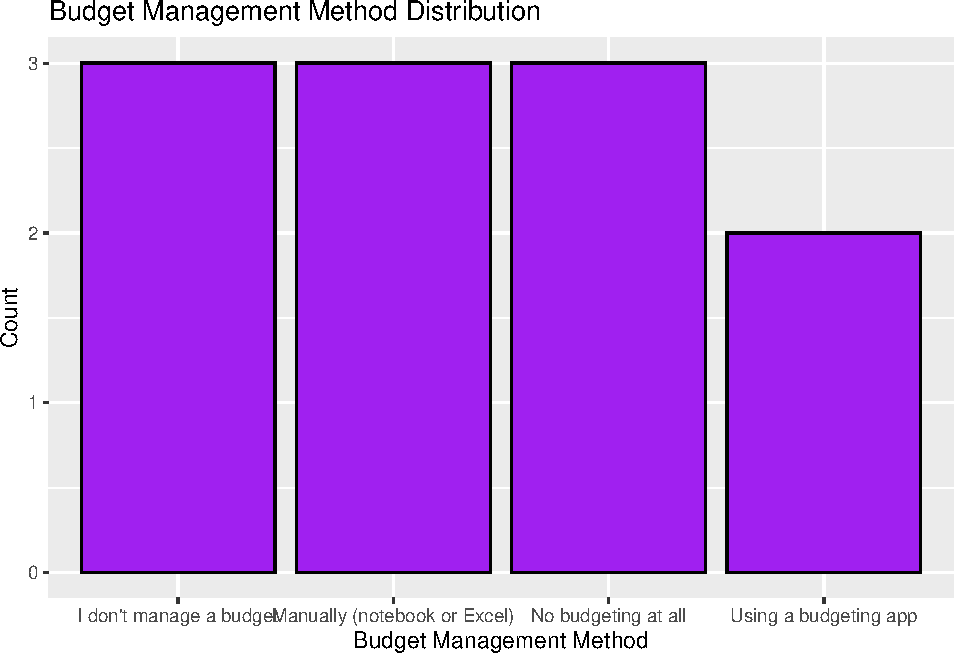
\includegraphics{Project1_files/figure-latex/unnamed-chunk-10-1.pdf}

\paragraph{Saving for Future Expenses vs.~Employment
Status}\label{saving-for-future-expenses-vs.-employment-status}

\begin{Shaded}
\begin{Highlighting}[]
\CommentTok{\# Bar Plot for Saving for Future Expenses vs. Employment Status}
\FunctionTok{ggplot}\NormalTok{(df, }\FunctionTok{aes}\NormalTok{(}\AttributeTok{x =} \FunctionTok{as.factor}\NormalTok{(Employment\_Status), }\AttributeTok{fill =} \FunctionTok{as.factor}\NormalTok{(Saving\_For\_Future\_Expenses))) }\SpecialCharTok{+}
  \FunctionTok{geom\_bar}\NormalTok{(}\AttributeTok{position =} \StringTok{"dodge"}\NormalTok{, }\AttributeTok{color =} \StringTok{"black"}\NormalTok{) }\SpecialCharTok{+}
  \FunctionTok{labs}\NormalTok{(}\AttributeTok{title =} \StringTok{"Saving for Future Expenses by Employment Status"}\NormalTok{, }\AttributeTok{x =} \StringTok{"Employment Status (0 = Unemployed, 1 = Employed)"}\NormalTok{, }\AttributeTok{y =} \StringTok{"Count"}\NormalTok{, }\AttributeTok{fill =} \StringTok{"Saving for Future Expenses (0 = No, 1 = Yes)"}\NormalTok{)}
\end{Highlighting}
\end{Shaded}

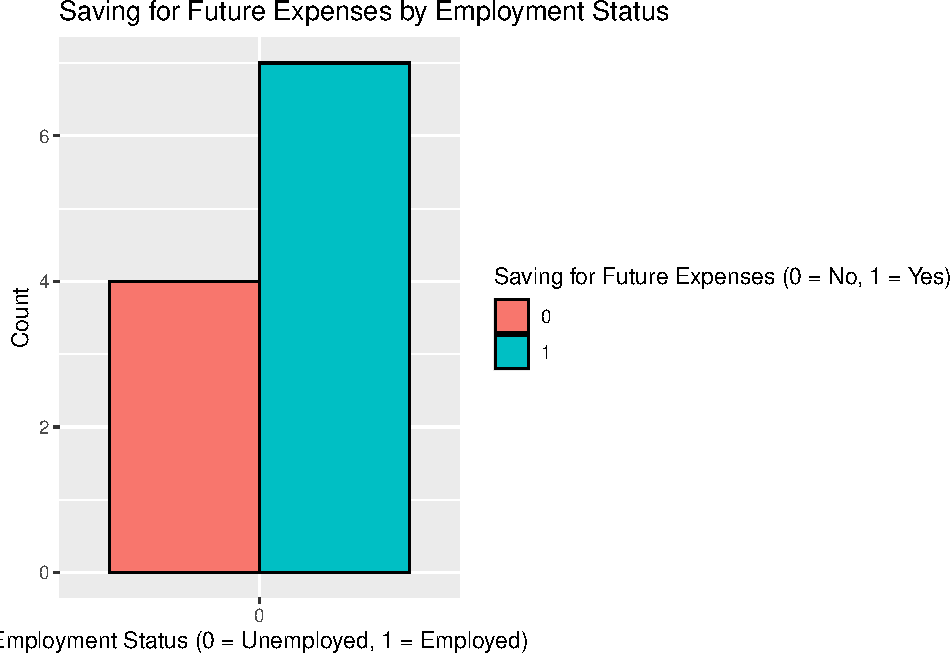
\includegraphics{Project1_files/figure-latex/unnamed-chunk-11-1.pdf}

\paragraph{Financial Independence Confidence by Employment
Status}\label{financial-independence-confidence-by-employment-status}

\begin{Shaded}
\begin{Highlighting}[]
\CommentTok{\# Bar Plot for Financial Independence Confidence by Employment Status}
\FunctionTok{ggplot}\NormalTok{(df, }\FunctionTok{aes}\NormalTok{(}\AttributeTok{x =} \FunctionTok{as.factor}\NormalTok{(Employment\_Status), }\AttributeTok{fill =} \FunctionTok{as.factor}\NormalTok{(Financial\_Independence\_Confidence))) }\SpecialCharTok{+}
  \FunctionTok{geom\_bar}\NormalTok{(}\AttributeTok{position =} \StringTok{"dodge"}\NormalTok{, }\AttributeTok{color =} \StringTok{"black"}\NormalTok{) }\SpecialCharTok{+}
  \FunctionTok{labs}\NormalTok{(}\AttributeTok{title =} \StringTok{"Financial Independence Confidence by Employment Status"}\NormalTok{, }\AttributeTok{x =} \StringTok{"Employment Status (0 = Unemployed, 1 = Employed)"}\NormalTok{, }\AttributeTok{y =} \StringTok{"Count"}\NormalTok{, }\AttributeTok{fill =} \StringTok{"Financial Independence Confidence (0 = Not Confident, 1 = Confident)"}\NormalTok{)}
\end{Highlighting}
\end{Shaded}

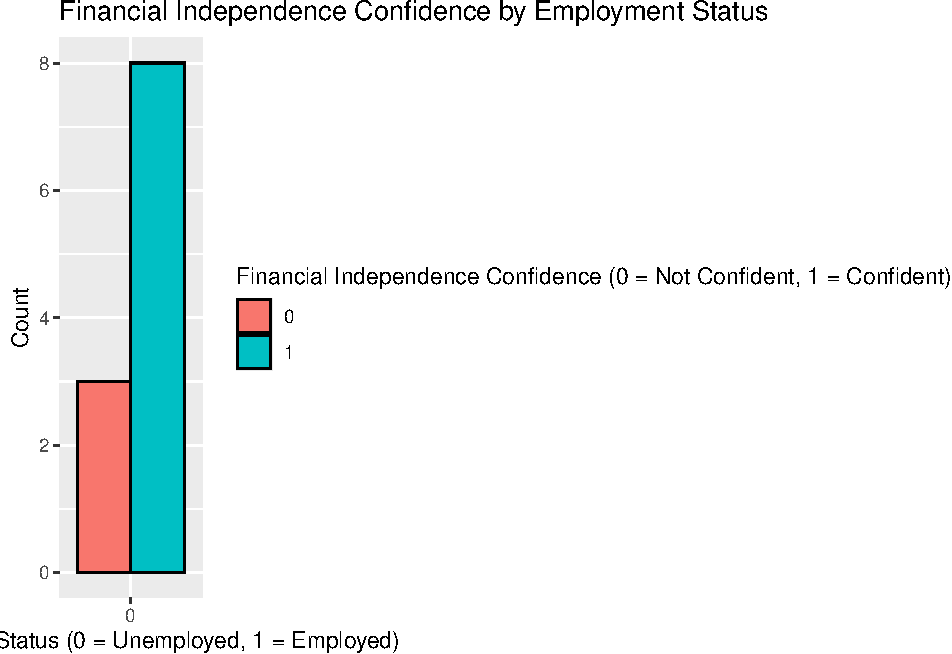
\includegraphics{Project1_files/figure-latex/unnamed-chunk-12-1.pdf}

\subsubsection{Word Cloud Analysis}\label{word-cloud-analysis}

\paragraph{Word Cloud for Future Financial Decision
Impact}\label{word-cloud-for-future-financial-decision-impact}

\begin{Shaded}
\begin{Highlighting}[]
\CommentTok{\# Create a Word Cloud for Future Financial Decision Impact}
\NormalTok{text\_data }\OtherTok{=} \FunctionTok{Corpus}\NormalTok{(}\FunctionTok{VectorSource}\NormalTok{(df}\SpecialCharTok{$}\NormalTok{Future\_Financial\_Decision\_Impact))}
\NormalTok{text\_data }\OtherTok{=}\NormalTok{ text\_data }\SpecialCharTok{\%\textgreater{}\%}
  \FunctionTok{tm\_map}\NormalTok{(}\FunctionTok{content\_transformer}\NormalTok{(tolower)) }\SpecialCharTok{\%\textgreater{}\%}
  \FunctionTok{tm\_map}\NormalTok{(removePunctuation) }\SpecialCharTok{\%\textgreater{}\%}
  \FunctionTok{tm\_map}\NormalTok{(removeNumbers) }\SpecialCharTok{\%\textgreater{}\%}
  \FunctionTok{tm\_map}\NormalTok{(removeWords, }\FunctionTok{stopwords}\NormalTok{(}\StringTok{"english"}\NormalTok{))}
\end{Highlighting}
\end{Shaded}

\begin{verbatim}
## Warning in tm_map.SimpleCorpus(., content_transformer(tolower)): transformation
## drops documents
\end{verbatim}

\begin{verbatim}
## Warning in tm_map.SimpleCorpus(., removePunctuation): transformation drops
## documents
\end{verbatim}

\begin{verbatim}
## Warning in tm_map.SimpleCorpus(., removeNumbers): transformation drops
## documents
\end{verbatim}

\begin{verbatim}
## Warning in tm_map.SimpleCorpus(., removeWords, stopwords("english")):
## transformation drops documents
\end{verbatim}

\begin{Shaded}
\begin{Highlighting}[]
\FunctionTok{wordcloud}\NormalTok{(text\_data, }\AttributeTok{max.words =} \DecValTok{100}\NormalTok{, }\AttributeTok{random.order =} \ConstantTok{FALSE}\NormalTok{, }\AttributeTok{colors =} \FunctionTok{brewer.pal}\NormalTok{(}\DecValTok{8}\NormalTok{, }\StringTok{"Dark2"}\NormalTok{))}
\end{Highlighting}
\end{Shaded}


\includegraphics{Project1_files/figure-latex/unnamed-chunk-13-1.pdf}

\subsection{Inferential Analysis}\label{inferential-analysis}

\subsubsection{Regression Analysis}\label{regression-analysis}

\paragraph{Predicting Financial
Confidence}\label{predicting-financial-confidence}

\begin{Shaded}
\begin{Highlighting}[]
\CommentTok{\# Linear Regression to Predict Financial Confidence}
\NormalTok{lm\_model }\OtherTok{=} \FunctionTok{lm}\NormalTok{(Financial\_Confidence }\SpecialCharTok{\textasciitilde{}}\NormalTok{ Employment\_Status }\SpecialCharTok{+}\NormalTok{ Student\_Loans }\SpecialCharTok{+}\NormalTok{ Saving\_For\_Future\_Expenses }\SpecialCharTok{+}\NormalTok{ Saving\_For\_Retirement, }\AttributeTok{data =}\NormalTok{ df)}
\FunctionTok{summary}\NormalTok{(lm\_model)}
\end{Highlighting}
\end{Shaded}

\begin{verbatim}
## 
## Call:
## lm(formula = Financial_Confidence ~ Employment_Status + Student_Loans + 
##     Saving_For_Future_Expenses + Saving_For_Retirement, data = df)
## 
## Residuals:
##     Min      1Q  Median      3Q     Max 
## -1.2857 -0.4286 -0.1429  0.7143  0.8571 
## 
## Coefficients: (1 not defined because of singularities)
##                             Estimate Std. Error t value Pr(>|t|)    
## (Intercept)                3.286e+00  4.860e-01   6.761 0.000262 ***
## Employment_Status                 NA         NA      NA       NA    
## Student_Loans              2.857e-01  7.769e-01   0.368 0.723902    
## Saving_For_Future_Expenses 2.012e-16  6.547e-01   0.000 1.000000    
## Saving_For_Retirement      8.571e-01  5.915e-01   1.449 0.190573    
## ---
## Signif. codes:  0 '***' 0.001 '**' 0.01 '*' 0.05 '.' 0.1 ' ' 1
## 
## Residual standard error: 0.9258 on 7 degrees of freedom
## Multiple R-squared:  0.2667, Adjusted R-squared:  -0.04762 
## F-statistic: 0.8485 on 3 and 7 DF,  p-value: 0.5099
\end{verbatim}

\subsubsection{Cross-Tabulations}\label{cross-tabulations}

\paragraph{Cross-Tabulation: Budgeting Method by Employment
Status}\label{cross-tabulation-budgeting-method-by-employment-status}

\begin{Shaded}
\begin{Highlighting}[]
\CommentTok{\# Cross{-}tabulation of Budgeting Method by Employment Status}
\NormalTok{budget\_vs\_employment }\OtherTok{=} \FunctionTok{table}\NormalTok{(df}\SpecialCharTok{$}\NormalTok{Budget\_Management\_Method, df}\SpecialCharTok{$}\NormalTok{Employment\_Status)}
\FunctionTok{print}\NormalTok{(budget\_vs\_employment)}
\end{Highlighting}
\end{Shaded}

\begin{verbatim}
##                               
##                                0
##   I don't manage a budget      3
##   Manually (notebook or Excel) 3
##   No budgeting at all          3
##   Using a budgeting app        2
\end{verbatim}

\paragraph{Cross-Tabulation: Financial Confidence by Saving
Habits}\label{cross-tabulation-financial-confidence-by-saving-habits}

\begin{Shaded}
\begin{Highlighting}[]
\CommentTok{\# Cross{-}tabulation of Financial Confidence by Saving for Future Expenses}
\NormalTok{confidence\_vs\_saving }\OtherTok{=} \FunctionTok{table}\NormalTok{(df}\SpecialCharTok{$}\NormalTok{Financial\_Confidence, df}\SpecialCharTok{$}\NormalTok{Saving\_For\_Future\_Expenses)}
\FunctionTok{print}\NormalTok{(confidence\_vs\_saving)}
\end{Highlighting}
\end{Shaded}

\begin{verbatim}
##    
##     0 1
##   2 1 0
##   3 0 3
##   4 3 2
##   5 0 2
\end{verbatim}

\subsubsection{Clustering Analysis}\label{clustering-analysis}

\paragraph{K-Means Clustering of Financial
Behaviors}\label{k-means-clustering-of-financial-behaviors}

\begin{Shaded}
\begin{Highlighting}[]
\CommentTok{\# K{-}Means Clustering}
\NormalTok{df\_numeric }\OtherTok{=}\NormalTok{ df }\SpecialCharTok{\%\textgreater{}\%} \FunctionTok{select\_if}\NormalTok{(is.numeric)}
\NormalTok{kmeans\_result }\OtherTok{=} \FunctionTok{kmeans}\NormalTok{(df\_numeric, }\AttributeTok{centers =} \DecValTok{3}\NormalTok{)}
\NormalTok{df}\SpecialCharTok{$}\NormalTok{Cluster }\OtherTok{=} \FunctionTok{as.factor}\NormalTok{(kmeans\_result}\SpecialCharTok{$}\NormalTok{cluster)}

\CommentTok{\# Plot Clustering Results with Circles}
\FunctionTok{ggplot}\NormalTok{(df, }\FunctionTok{aes}\NormalTok{(}\AttributeTok{x =}\NormalTok{ Financial\_Confidence, }\AttributeTok{y =}\NormalTok{ Student\_Debt\_Concern, }\AttributeTok{color =}\NormalTok{ Cluster)) }\SpecialCharTok{+}
  \FunctionTok{geom\_point}\NormalTok{() }\SpecialCharTok{+}
  \FunctionTok{stat\_ellipse}\NormalTok{(}\FunctionTok{aes}\NormalTok{(}\AttributeTok{group =}\NormalTok{ Cluster), }\AttributeTok{type =} \StringTok{"norm"}\NormalTok{, }\AttributeTok{linetype =} \DecValTok{2}\NormalTok{) }\SpecialCharTok{+}
  \FunctionTok{labs}\NormalTok{(}\AttributeTok{title =} \StringTok{"K{-}Means Clustering of Financial Behaviors"}\NormalTok{, }\AttributeTok{x =} \StringTok{"Financial Confidence"}\NormalTok{, }\AttributeTok{y =} \StringTok{"Student Debt Concern"}\NormalTok{, }\AttributeTok{color =} \StringTok{"Cluster"}\NormalTok{)}
\end{Highlighting}
\end{Shaded}

\begin{verbatim}
## Too few points to calculate an ellipse
\end{verbatim}

\begin{verbatim}
## Warning: Removed 1 row containing missing values or values outside the scale range
## (`geom_path()`).
\end{verbatim}

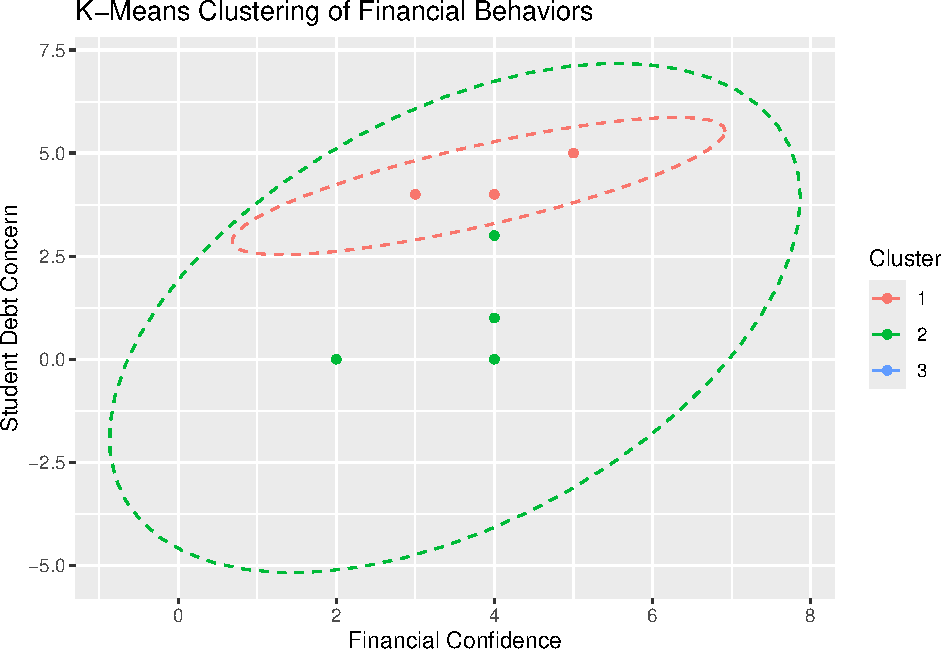
\includegraphics{Project1_files/figure-latex/unnamed-chunk-17-1.pdf}

\subsubsection{Percentage Analysis of Survey
Responses}\label{percentage-analysis-of-survey-responses}

\begin{Shaded}
\begin{Highlighting}[]
\CommentTok{\# Percentage of Responses for Key Questions}

\CommentTok{\# Percentage of Students with Student Loans}
\NormalTok{total\_responses }\OtherTok{=} \FunctionTok{nrow}\NormalTok{(df)}
\NormalTok{students\_with\_loans }\OtherTok{=} \FunctionTok{sum}\NormalTok{(df}\SpecialCharTok{$}\NormalTok{Student\_Loans }\SpecialCharTok{==} \DecValTok{1}\NormalTok{)}
\NormalTok{percentage\_loans }\OtherTok{=}\NormalTok{ (students\_with\_loans }\SpecialCharTok{/}\NormalTok{ total\_responses) }\SpecialCharTok{*} \DecValTok{100}
\FunctionTok{cat}\NormalTok{(}\StringTok{"Percentage of students with student loans:"}\NormalTok{, percentage\_loans, }\StringTok{"\%}\SpecialCharTok{\textbackslash{}n}\StringTok{"}\NormalTok{)}
\end{Highlighting}
\end{Shaded}

\begin{verbatim}
## Percentage of students with student loans: 18.18182 %
\end{verbatim}

\begin{Shaded}
\begin{Highlighting}[]
\CommentTok{\# Percentage of Students Saving for Future Expenses}
\NormalTok{saving\_for\_expenses }\OtherTok{=} \FunctionTok{sum}\NormalTok{(df}\SpecialCharTok{$}\NormalTok{Saving\_For\_Future\_Expenses }\SpecialCharTok{==} \DecValTok{1}\NormalTok{)}
\NormalTok{percentage\_saving\_expenses }\OtherTok{=}\NormalTok{ (saving\_for\_expenses }\SpecialCharTok{/}\NormalTok{ total\_responses) }\SpecialCharTok{*} \DecValTok{100}
\FunctionTok{cat}\NormalTok{(}\StringTok{"Percentage of students saving for future expenses:"}\NormalTok{, percentage\_saving\_expenses, }\StringTok{"\%}\SpecialCharTok{\textbackslash{}n}\StringTok{"}\NormalTok{)}
\end{Highlighting}
\end{Shaded}

\begin{verbatim}
## Percentage of students saving for future expenses: 63.63636 %
\end{verbatim}

\begin{Shaded}
\begin{Highlighting}[]
\CommentTok{\# Percentage of Students Saving for Retirement}
\NormalTok{saving\_for\_retirement }\OtherTok{=} \FunctionTok{sum}\NormalTok{(df}\SpecialCharTok{$}\NormalTok{Saving\_For\_Retirement }\SpecialCharTok{==} \DecValTok{1}\NormalTok{)}
\NormalTok{percentage\_saving\_retirement }\OtherTok{=}\NormalTok{ (saving\_for\_retirement }\SpecialCharTok{/}\NormalTok{ total\_responses) }\SpecialCharTok{*} \DecValTok{100}
\FunctionTok{cat}\NormalTok{(}\StringTok{"Percentage of students saving for retirement:"}\NormalTok{, percentage\_saving\_retirement, }\StringTok{"\%}\SpecialCharTok{\textbackslash{}n}\StringTok{"}\NormalTok{)}
\end{Highlighting}
\end{Shaded}

\begin{verbatim}
## Percentage of students saving for retirement: 45.45455 %
\end{verbatim}

\begin{Shaded}
\begin{Highlighting}[]
\CommentTok{\# Percentage of Employed Students}
\NormalTok{employed\_students }\OtherTok{=} \FunctionTok{sum}\NormalTok{(df}\SpecialCharTok{$}\NormalTok{Employment\_Status }\SpecialCharTok{==} \DecValTok{1}\NormalTok{)}
\NormalTok{percentage\_employed }\OtherTok{=}\NormalTok{ (employed\_students }\SpecialCharTok{/}\NormalTok{ total\_responses) }\SpecialCharTok{*} \DecValTok{100}
\FunctionTok{cat}\NormalTok{(}\StringTok{"Percentage of students employed while attending school:"}\NormalTok{, percentage\_employed, }\StringTok{"\%}\SpecialCharTok{\textbackslash{}n}\StringTok{"}\NormalTok{)}
\end{Highlighting}
\end{Shaded}

\begin{verbatim}
## Percentage of students employed while attending school: 0 %
\end{verbatim}

\begin{Shaded}
\begin{Highlighting}[]
\CommentTok{\# Percentage of Students Confident in Financial Independence}
\NormalTok{confident\_financial\_independence }\OtherTok{=} \FunctionTok{sum}\NormalTok{(df}\SpecialCharTok{$}\NormalTok{Financial\_Independence\_Confidence }\SpecialCharTok{==} \DecValTok{1}\NormalTok{)}
\NormalTok{percentage\_confident\_independence }\OtherTok{=}\NormalTok{ (confident\_financial\_independence }\SpecialCharTok{/}\NormalTok{ total\_responses) }\SpecialCharTok{*} \DecValTok{100}
\FunctionTok{cat}\NormalTok{(}\StringTok{"Percentage of students confident in achieving financial independence:"}\NormalTok{, percentage\_confident\_independence, }\StringTok{"\%}\SpecialCharTok{\textbackslash{}n}\StringTok{"}\NormalTok{)}
\end{Highlighting}
\end{Shaded}

\begin{verbatim}
## Percentage of students confident in achieving financial independence: 72.72727 %
\end{verbatim}

\begin{Shaded}
\begin{Highlighting}[]
\CommentTok{\# Percentage of Students Confident in Job Post Graduation}
\NormalTok{confident\_job\_post\_graduation }\OtherTok{=} \FunctionTok{sum}\NormalTok{(df}\SpecialCharTok{$}\NormalTok{Job\_Confidence\_Post\_Graduation }\SpecialCharTok{==} \DecValTok{1}\NormalTok{)}
\NormalTok{percentage\_confident\_job }\OtherTok{=}\NormalTok{ (confident\_job\_post\_graduation }\SpecialCharTok{/}\NormalTok{ total\_responses) }\SpecialCharTok{*} \DecValTok{100}
\FunctionTok{cat}\NormalTok{(}\StringTok{"Percentage of students confident in finding a job post{-}graduation:"}\NormalTok{, percentage\_confident\_job, }\StringTok{"\%}\SpecialCharTok{\textbackslash{}n}\StringTok{"}\NormalTok{)}
\end{Highlighting}
\end{Shaded}

\begin{verbatim}
## Percentage of students confident in finding a job post-graduation: 63.63636 %
\end{verbatim}

\subsubsection{Additional EDA
Suggestions}\label{additional-eda-suggestions}

\paragraph{Heatmap of Correlations}\label{heatmap-of-correlations}

\begin{Shaded}
\begin{Highlighting}[]
\CommentTok{\# Heatmap of Correlations to visualize relationships between variables}
\FunctionTok{ggcorrplot}\NormalTok{(correlation\_matrix, }\AttributeTok{method =} \StringTok{"circle"}\NormalTok{, }\AttributeTok{type =} \StringTok{"lower"}\NormalTok{, }\AttributeTok{lab =} \ConstantTok{TRUE}\NormalTok{, }\AttributeTok{title =} \StringTok{"Heatmap of Correlations"}\NormalTok{)}
\end{Highlighting}
\end{Shaded}

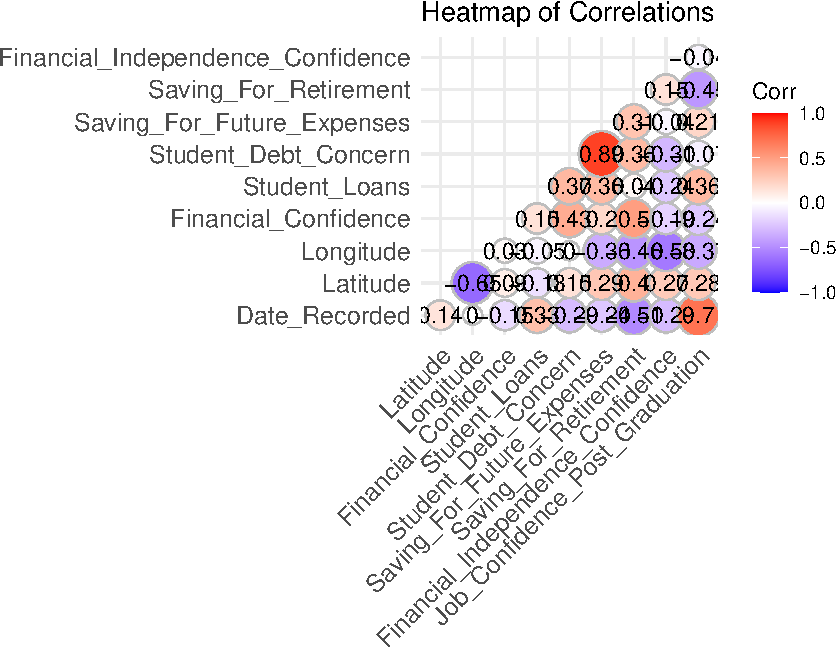
\includegraphics{Project1_files/figure-latex/unnamed-chunk-19-1.pdf}

\paragraph{Boxplots for Spending
Habits}\label{boxplots-for-spending-habits}

\begin{Shaded}
\begin{Highlighting}[]
\CommentTok{\# Boxplot for Biggest Expense Categories}
\FunctionTok{ggplot}\NormalTok{(df, }\FunctionTok{aes}\NormalTok{(}\AttributeTok{x =}\NormalTok{ Biggest\_Expense, }\AttributeTok{y =}\NormalTok{ Financial\_Confidence)) }\SpecialCharTok{+}
  \FunctionTok{geom\_boxplot}\NormalTok{(}\AttributeTok{fill =} \StringTok{"lightblue"}\NormalTok{, }\AttributeTok{color =} \StringTok{"black"}\NormalTok{) }\SpecialCharTok{+}
  \FunctionTok{labs}\NormalTok{(}\AttributeTok{title =} \StringTok{"Boxplot of Financial Confidence by Biggest Expense"}\NormalTok{, }\AttributeTok{x =} \StringTok{"Biggest Expense"}\NormalTok{, }\AttributeTok{y =} \StringTok{"Financial Confidence"}\NormalTok{)}
\end{Highlighting}
\end{Shaded}

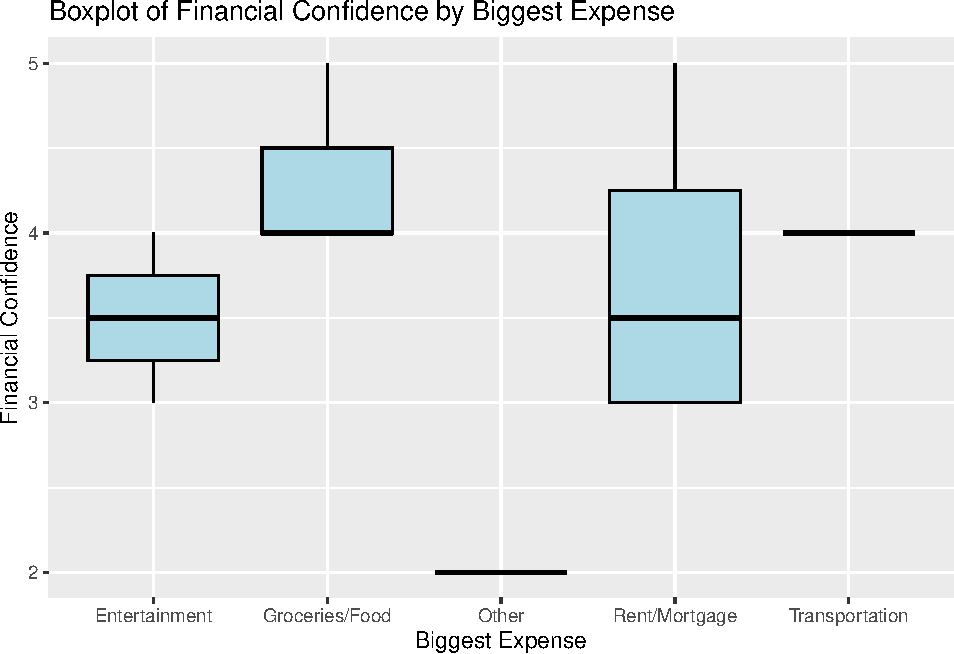
\includegraphics{Project1_files/figure-latex/unnamed-chunk-20-1.pdf}

\subsubsection{Geographic Analysis Using
Mapview}\label{geographic-analysis-using-mapview}

\#\texttt{\{r\}\ \#library(mapview)\ \#\ Plot\ the\ locations\ using\ mapview\ \#mapview(df,\ xcol\ =\ "Longitude",\ ycol\ =\ "Latitude",\ crs\ =\ 4269,\ grid\ =\ FALSE)\ \#}

\end{document}
